\documentclass[journal]{IEEEtran}
\usepackage{enumerate} 
\usepackage[spanish,activeacute]{babel}
\usepackage{graphicx}
\usepackage[latin1]{inputenc}

\hyphenation{op-tical net-works semi-conduc-tor}


\begin{document}
\title{Encendido de 5 luces y luz parpadeante.}
\author{Pedro A. Moreno \\
Departamento de Estudios Multidisciplinarios, Campus Irapuato Salamanca, Universidad de Guanajuato, Yuriria, Guanajuato, M\'exico. \\
Email: pa.morenovazquez@ugto.mx

\thanks{Marzo 14, 2017}}
\markboth{Micrioprocesadores y Microcontroladres,  Febrero~2017}%
{Shell \MakeLowercase{\textit{et al.}}: Bare Demo of IEEEtran.cls for IEEE Journals}



\maketitle

\begin{abstract}

Se uso un microcontrolador PIC 16f84A de microchip, con el fin encender un juego de 5 LED con 5 entradas y tener un led que parpadee con una frecuencia de un segundo.
Introducci�n 


\end{abstract}

%\begin{IEEEkeywords}
%IEEE, IEEEtran, journal, \LaTeX, paper, template.
%\end{IEEEkeywords}

\IEEEpeerreviewmaketitle

\section{Introducci\'on }

\IEEEPARstart{E}{l} PIC 16F84A contiene dos puertos de entrada o salida, A(5 bits) y B( bits), los cuales pueden ser usados para tener una salida cuyos resultados sean exactamente iguales a una entrada, pero para tener una salida no es absolutamente necesario el tener una entrada pues el microcontraldor puede ser �til para mostrar salidas.
\section{Metodolog\'ia }

\subsubsection{Materiales}
\begin{itemize}
	\item 1 PIC 16F84A.
    \item 1 mini dip switch de 8 pines.
    \item 5 LED.
    \item 5 resistencias de 300 $\Omega$.
    \item 5 resistencias de 100 $k   {  }\Omega$.
    \item Fuente de alimentaci�n.
\end{itemize}


\subsubsection{Desarrollo}

Para poder pasar la entrada dada a la salida es necesario poner la entrada en el registro de trabajo del micro controlador y del registro de trabajo pasarlo a la salida, estos procesos se repitiran hasta que el usuario decida terminar el proceso.

Para poder hacer un led o juego de ellos de forma intermitente es necesario tener una rutina el cual lleve un tiempo sucifiencte para notar notar el efecto deseado el cual, en este caso, es un segundo. Para lograr esto se tiene un ciclo el cual decremento un registro que comienza en 30, este decrementa un registro que comienza en 100, y este decremento un ciclo que comienza en 100, para obtener el tiempo total, $t$, se utiliza la ecuaci�n,

\begin{equation}\label{eq:m}
3(a+ab+abc)= t
\end{equation}

, donde $a$, $b$ y $c$ son los n�meros en que comenzaron los ciclos, en este caso se obtiene un tiempo 909090 microsegundos, se puede aumentar el numero de ciclo para aumentar la precisi�n y obtener un tiempo mas exacto a la interpretaci�n actual, y probablemente definitiva, del tiempo.
Ya obtenida la rutina de tiempo es necesario encender los leds, seguir con una rutina de tiempo, apagar los leds y otra rutina de tiempo para conformar as� un ciclo que parpadea un LED.

\begin{figure}
  \centering
    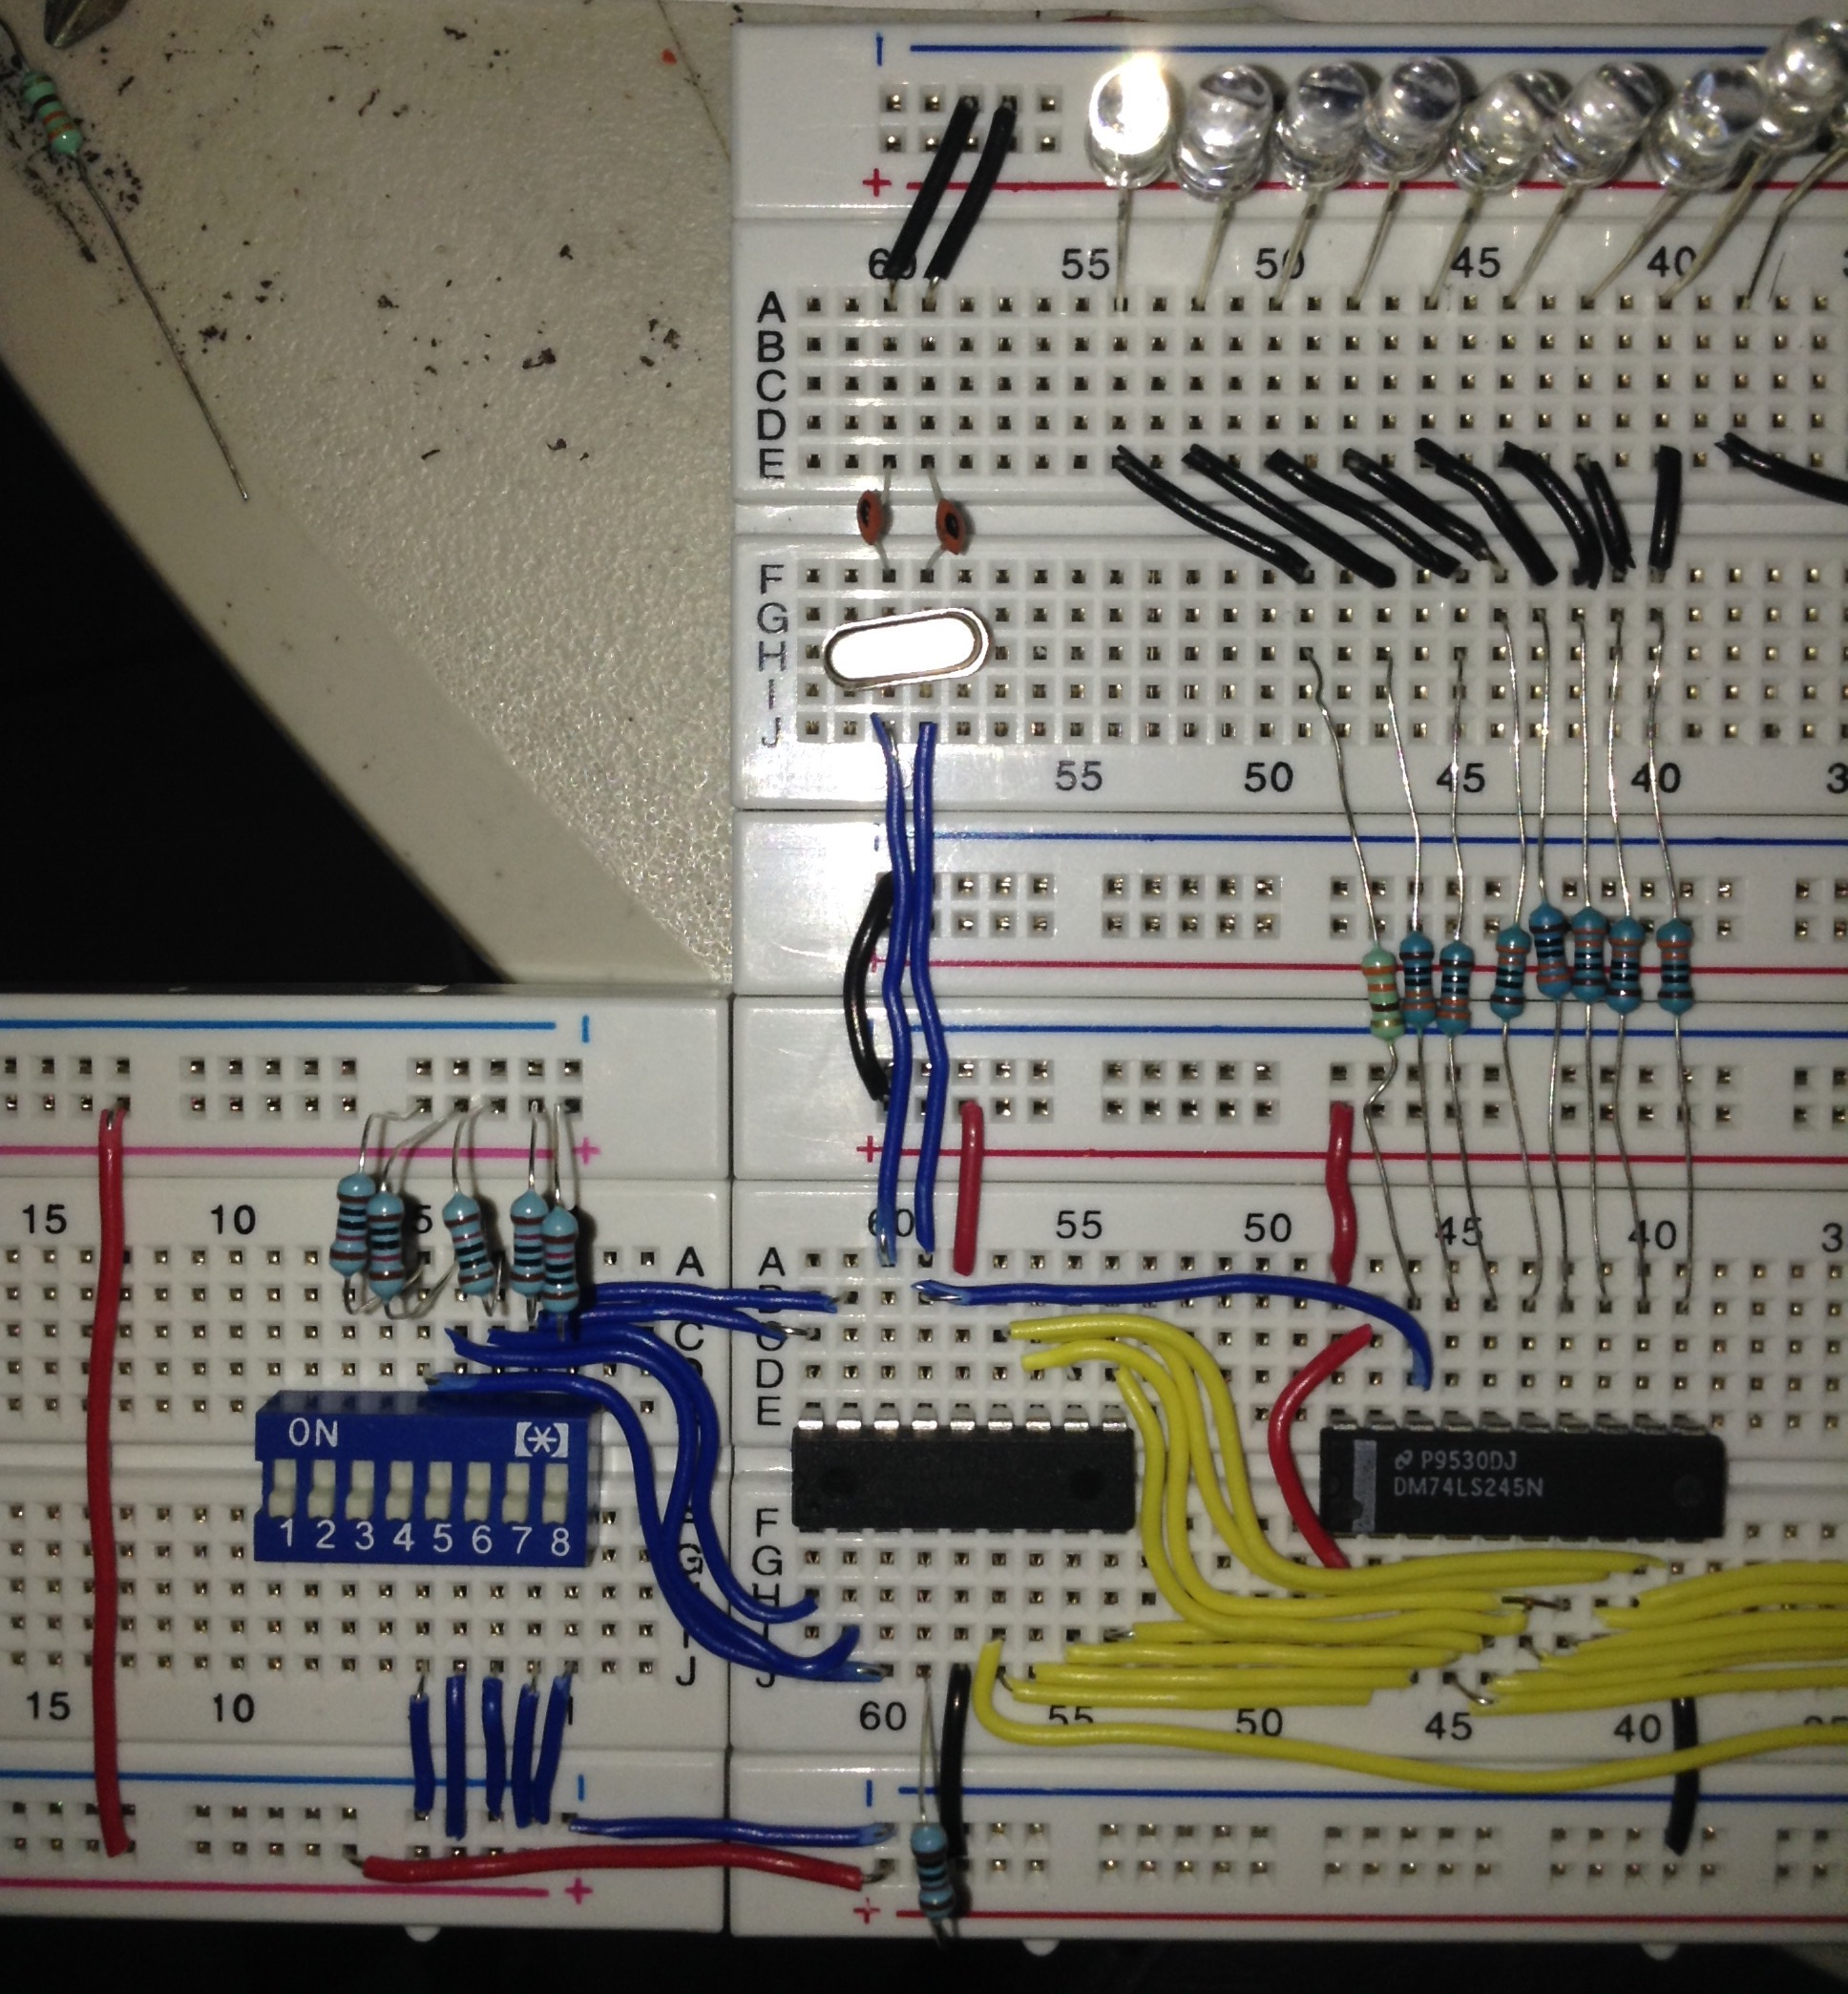
\includegraphics[width=0.45\textwidth]{FullSizeRender2.jpg}
  \caption{Circuito.}
  \label{calentrada}
\end{figure}




 
\section{Resultados }

En el primer objetivo los LED se encend�an al ritmo que el usuario deseaba sin complicaci�n alguna.
En el led parpadeante se obtuvo un LED cuyo encendido y apagado era notable para el ojo humano, pues 909090 microsegundos era mas que suficiente para este.

\section{Conclusi\'on }

Es interesante comprobar que el microcontrolador puede recibir entradas y obtener salidas, o solo obtener salidas directamente del microcontrolador, ademas en las rutinas de tiempo, como el microcontrolador trabaja secuencialmente, es interesante que toda acci�n le afecta a la definici�n de un segundo al sistema que se le da al sistema.



\end{document}